\chapter{Моделирование TGE и TGF
}\label{ch:thunderstorm}

\section{О высокоэнергетичном излучении в грозовых облаках}\label{sec:thunderstorm/review}
Ещё в 1925 году Уилсон~\cite{wilson1925acceleration} предсказывает что электроны проходящие через электрическое поле грозовых облаков должны ускорятся и излучать тормозное излучение, однако дальнейшее развитие этой идеи и экспериментальные наблюдения начались только в 90-ых годах XX века. Впервые TGF (Terrestrial gamma-ray flash) --- короткие (от 7 мкс до 3.5 мс) вспышки гамма- и рентгеновского излучения происходящие из земной атмосферы и ассоциированные с процессами происходящими в грозовых облаках, наблюдались в 1994 в эксперименте BATSE на спутнике CGRO (Compton Gamma Ray Observatory)~\cite{Fishman1313} принадлежащем NASA. В дальнейшем TGF также наблюдались на других космических обсерваториях NASA, таких как Fermi Gamma-ray Space Telescope~\cite{briggs2010first} и Ramaty High Energy Solar Spectroscopic Imager~\cite{Smith1085}. В 2018 году наблюдения подтверждаются также Итальянским космическим агентством проведшим анализ данных с космического аппарата AGILE (Astro-rivelatore Gamma a Immagini LEggero)~\cite{lindanger2018search}. Появились также и данные наземных наблюдений, например с российской станции на Тянь-Шане принадлежащей ФИАН им. Лебедева и армянской станции на г. Арагац принадлежащей Ереванскому физическому институту. Наблюдения на Тянь-Шане производятся на высоте от 3300 до 3800 метров над уровнем моря и благодаря такой близости к грозовым облакам дают широкий спектр данных: регистрация рентгеновского излучения от облаков~\cite{chubenko2000} во время грозы, рост числа регистрируемых электронов~\cite{chubenko2003}, измерение энергетических спектров TGF~\cite{chubenko2009, gurevich2011effective}, радионаблюдение ШАЛ проходящих через грозовые облака~\cite{antonova2007, antonova2009, gurevich2002radio, gurevich2003radio}, корреляцию гамма-вспышек и радиоизлучения при возникновении молнии~\cite{gurevich2013correlation}. Наблюдения на г. Арагац производятся с научной станции расположенной на высоте 3250 метров над уровнем моря, что позволяет производить измерения в непосредственной близости от облаков. В частности научная аппаратура станции позволяет регистрировать возрастание потоков гамма-квантов, электронов и нейтронов, вызванное грозовыми облаками, в том числе регистрируя электроны и гамма-кванты с энергиями до нескольких десятков МэВ, а также наблюдения на г. Арагац позволили описать TGE (Thunderstrom Ground Enhancements) --- длительное (по сравнению с TGF) увеличение потоков релятивистских частиц от грозовых облаков, ассоциированные с изменениями приземного электрического поля и достигающих максимальных значений одновременно с появлениям разрядов в облаке~\cite{PhysRevD.83.062001, PhysRevD.82.043009}. Что касается теоретического описания, то фундаментальной основой для описания этих экспериментальных наблюдений является пробой на убегающих электронах (ПУЭ) --- модель развития лавины релятивистских (с энергией 0.1 --- 10 МэВ) электронов в постоянном электрическом поле предложенная А.~В.~Гуревичем~\cite{gurevich1992runaway,Gurevich2001ufn}. Качественно идея модели проста: пусть электрон ускоряется за счет электрического поля и тормозится за счет взаимодействия со средой, если он получает от поля больше энергии чем теряет, то у него появляется избыток энергии, который может быть потрачен на рождение нового электрона. Такие электроны будем называть убегающими. Если пренебречь всеми процессами кроме ионизационных потерь и радиационных потерь, то график ~\ref{fig:storm:gurevich}а показывает условия для убегания. Энергию достаточную для убегания, то есть ту при которой электрон в среднем на единице длинны приобретает энергии больше чем теряет, мы будем называть критической (обозначена красной линией на графике ~\ref{fig:storm:gurevich}а, её зависимость  от высоты, полученная на основе величины ионизационных потерь, приведена на рис. ~\ref{fig:storm:gurevich}б). Таким образом электроны в поле выше предельного (черная линия на графике ~\ref{fig:storm:gurevich}а) с энергиями выше критической рождают новые электроны и образуют так называемую лавину убегающих электронов. 
%
\begin{figure}[t]
    \begin{center}
        \begin{minipage}[h]{0.49\linewidth}
            \center{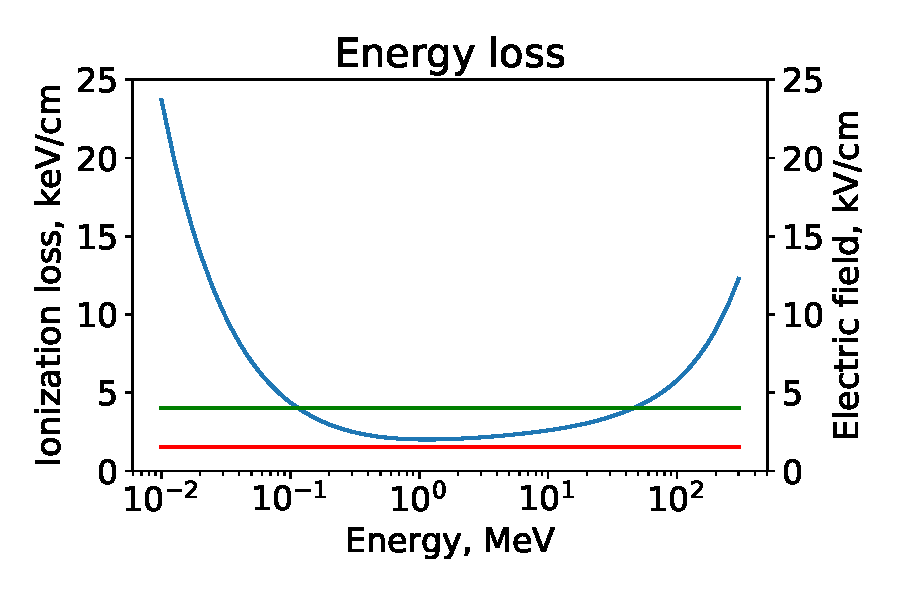
\includegraphics[width=\linewidth]{thunderstorm/01_Gurevich.pdf} \\ а)}
        \end{minipage}
        \hfill
        \begin{minipage}[h]{0.49\linewidth}
            \center{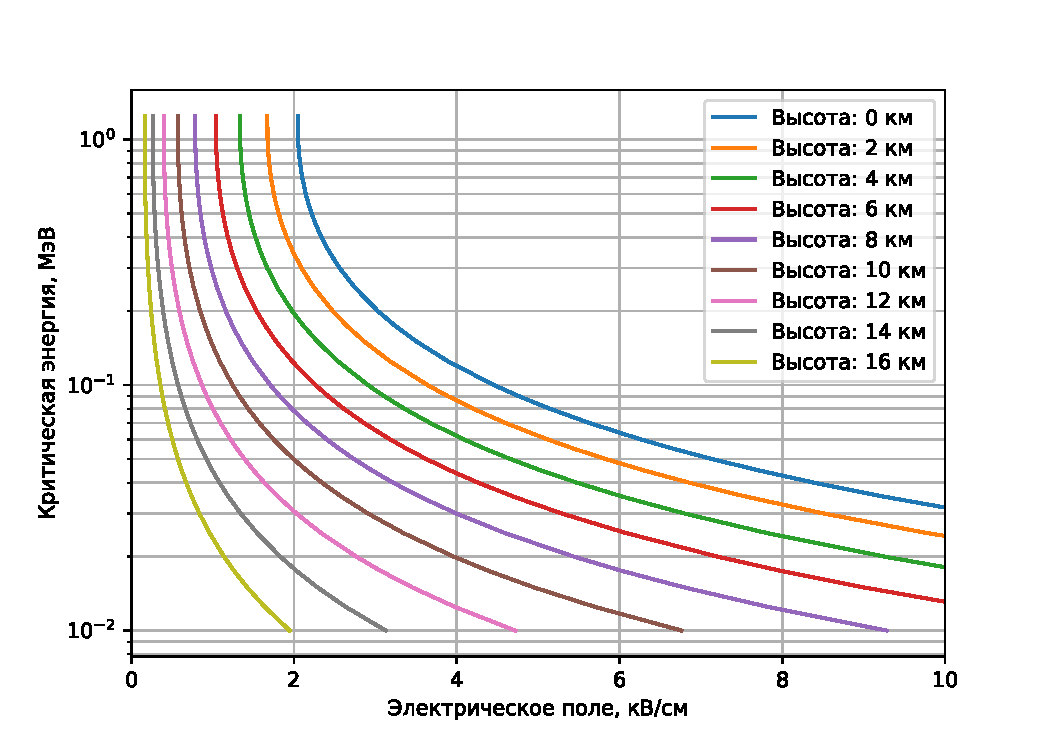
\includegraphics[width=\linewidth]{thunderstorm/02_CriticalEnergy.pdf}   \\ б)}
        \end{minipage}
        \caption{а) Ионизационные потери электронов в воздухе при нормальных условиях. б) Зависимость критической энергии от поля для различных высот.}
    \end{center}
    \label{fig:storm:gurevich}
\end{figure}
Конечно реальная структура модели является более сложной так как необходимо учитывать прочие процессы происходящие с электронами (см. раздел~\ref{sec:theory/propagation}), кроме того существуют разные способы попытаться построить модель пробоя: это можно делать как с помощью построения кинетической теории, как в работах~\ref{gurevich1992runaway,Gurevich2001ufn}, так и используя Монте-Карло моделирование как например в данной работе или в работе~\cite{dwyer2003fundamental}. Однако даже качественное описание позволяет нам предсказать следующие возможности:
\begin{itemize}
   \item Число убегающих электронов потенциально может оказаться настолько велико что вызовет пробой.
   \item Электроны в лавине в следствии ионизации производят большое количество тепловых электронов что влияет на проводящие характеристики облака, что в конечном итоге может привести к пробою.
   \item Убегающие электроны рождают не только новые убегающие электроны, но и гамма-кванты, которые могут быть источником TGF и TGE, а также приводить к некоторым другим эффектам.
\end{itemize}
Далее в работе мы рассмотрим как из моделирования можно получить количественные параметры лавин убегающих электронов, какое дальнейшее развитие имеет модель Гуревича, в чем проблемы некоторых моделей развивающих модель Гуревича, приведем описание нашей собственной концепции развивающую модель Гуревича для описания TGF и TGE, как лавины убегающих электронов можно использовать для изучения структуры облака и обсудим некоторые практические вопросы связанные с регистрацией нейтронов от TGF. Но перед этим мы укажем на некоторые особенности связанные с нашим Монте-Карло моделированием.


% Gurevich2000.pdf --- даны оценки числа рожденных электрон-позитронных пар
% Gurevich_etal2013.pdf gurevich2013correlation - Приведены результаты одновременных измерений радио и гамма-излучения во время гроз. Гамма-детектор, расположенный на высоте 3840 м, и два радиодетектора Тянь-Шаньской горной научной станции (высота 3340 м) регистрировали интенсивные гамма-вспышки и радиоимпульсы в момент возникновения молнии. В начальный момент времени (несколько сотен микросекунд) радиогамма-корреляция резко нарастает, а коэффициент корреляции достигает 0,9–0,95. Спектр гамма-энергии, измеренный при возникновении молнии, близок к характерному спектру пробоя на убегающих электронах. Наблюдаемые при этом радиоимпульсы имеют наибольшую амплитуду. Совместное наблюдение гамма-излучения и радиоизлучения подтверждает концепцию возникновения молнии из-за множественных одновременных электрических разрядов на гидрометеорах, стимулированных и синхронизированных низкоэнергетическими электронами, генерируемыми в процессе разгона. 

% Gurevich2001.pdf -- рсчеты гуревича для неоднороного поля, добавить в раздел про реактор


%\section{Пробой на убегающих электронах}
%\label{sec:thunderstorm/gurevich}

\section{Особенности GEANT4 моделирования лавин убегающих электронов}\label{sec:thunderstorm/geant4}
В данном разделе указанны некоторые замечания касательно особенностей GEANT4 моделирования лавин убегающих электронов.
Во-первых, как обсуждалось в разделе~\ref{sec:theory/models}, есть отличия в результатах моделирования для разных физических листов в зависимости от версии GEANT4. Для более поздних версий характерно сокращения отличий в результатах моделирования для разных физических листов, для более характерно что менее точные (и за счет этого более быстрые) физические листы дают большое число убегающих электронов в лавине, как например на рис.~\ref{}\todo{ссылка на рисунок}. Таким образом получаем сверху на число убегающих электронов, других частиц и ионизацию облака, это нас вполне устраивает поскольку такая оценка позволяет сказать являются ли процессы связанные с убегающими электронами существенными для грозовых процессов в атмосфере.
Во-вторых, при моделировании убегающих электронов возникает проблема что в лавина одновременно содержит большое количество частиц, которое не помещается в оперативную память компьютера, однако эту проблему можно частично решить используя механизмы распределения по стекам очередности (сами стеки описаны в разделе~\ref{sec:theory/geant4}). При этом используется следующая логика: частицы производят очень разное количество вторичных частиц, и если не регулировать порядок симуляции может оказаться так что у нас закончится память для сохранения новых частиц в то время как в памяти скопиться много частиц, которые вообще могут не давать вторичных частиц и которые нам бы надо было бы смоделировать что бы очистить память. Что бы избегать таких ситуаций были введены критерии распределяющие частицы по стекам определяющим очередность симуляции, при этом использовались следующие соображения:
\begin{itemize}
   \item В отличии от заряженных частиц гамма-квант не способен получать энергию от электрического поля облака и число вторичных электронов ограничено полной энергией гамма-кванта, в то время как число вторичных частиц от убегающего электрона/позитрона ограниченно только размерами облака и величиной поля.
   \item Частицы с малыми, близки к критической энергиями имеют малый шанс породить вторичную частицы.
   \item Позитроны фактически создают новую лавину, поэтому они моделируются  в последнюю очередь, после того как смоделирована начальная лавина.
\end{itemize}
На основании этого была выстроена следующая очерёдность:
\begin{itemize}
    \item Гамма-кванты с энергиями меньше 0.08 МэВ.
    \item Электроны с энергиями меньше 0.08 МэВ.
    \item Гамма-кванты с энергиями меньше 0.5 МэВ.
    \item Остальные гамма-кванты.
    \item Остальные электроны.
    \item Позитроны.
\end{itemize}
В-третьих, существенную роль играет нижний порог для моделирования, так как велико число низкоэнергитичных частиц, недоучет этих частиц с одной стороны приводит к неправильной оценке числа электронов в лавине и ионизации облака, с другой стороны недостаточно агрессивное отрезание частиц по энергии приводит к истощению вычислительных ресурсов. Поэтому что бы уточнить значение критической энергии проведено отдельно Монте-Карло моделирование и сравнено с результатами оценки критической энергии только по ионизационным потерям (результат см. на рис.~\ref{fig:storm:simcrit}). Как мы видим значение критической энергии по моделированию не много выше чем оценка по ионизационным потерям, что позволяет нам установить порог частиц равным критической энергии ионизационным потерям не боясь недооценить число частиц в лавине.
Если не сказано иное, результат моделирования приводятся нормированным на число первичных частиц. Моделирование проводилось для облаков на различных высотах при этом для установления значения плотности воздуха на данной высоте используется международная стандартная модель атмосферы (ГОСТ 4401-81). Прочие параметры такие, как форма облака и размер поля приводятся при описании симуляции.


\begin{figure}[t]
    \begin{center}
        \begin{minipage}[h]{0.49\linewidth}
            \center{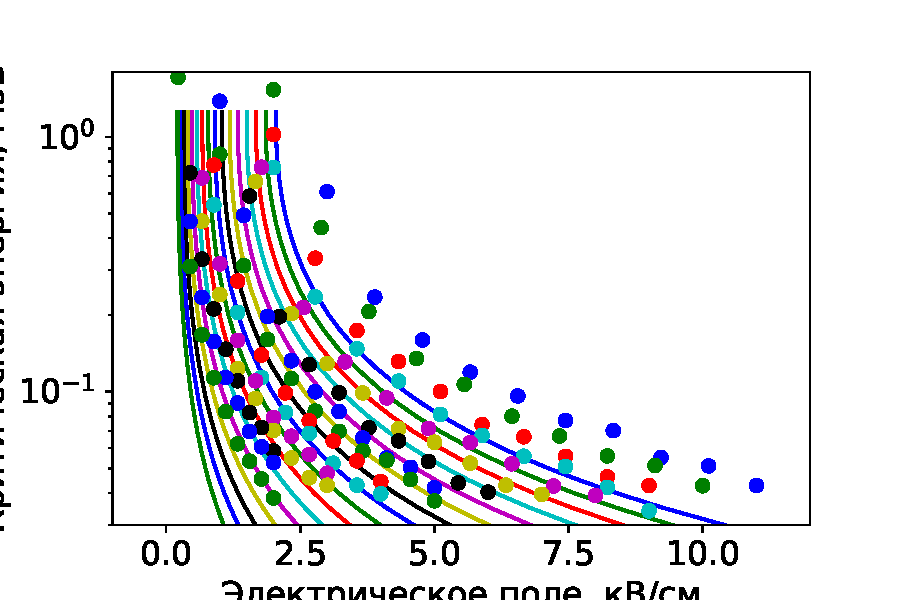
\includegraphics[width=\linewidth]{thunderstorm/03_CriticalEnergyWithSim.pdf} \\ а)}
        \end{minipage}
        \hfill
        \begin{minipage}[h]{0.49\linewidth}
            %\center{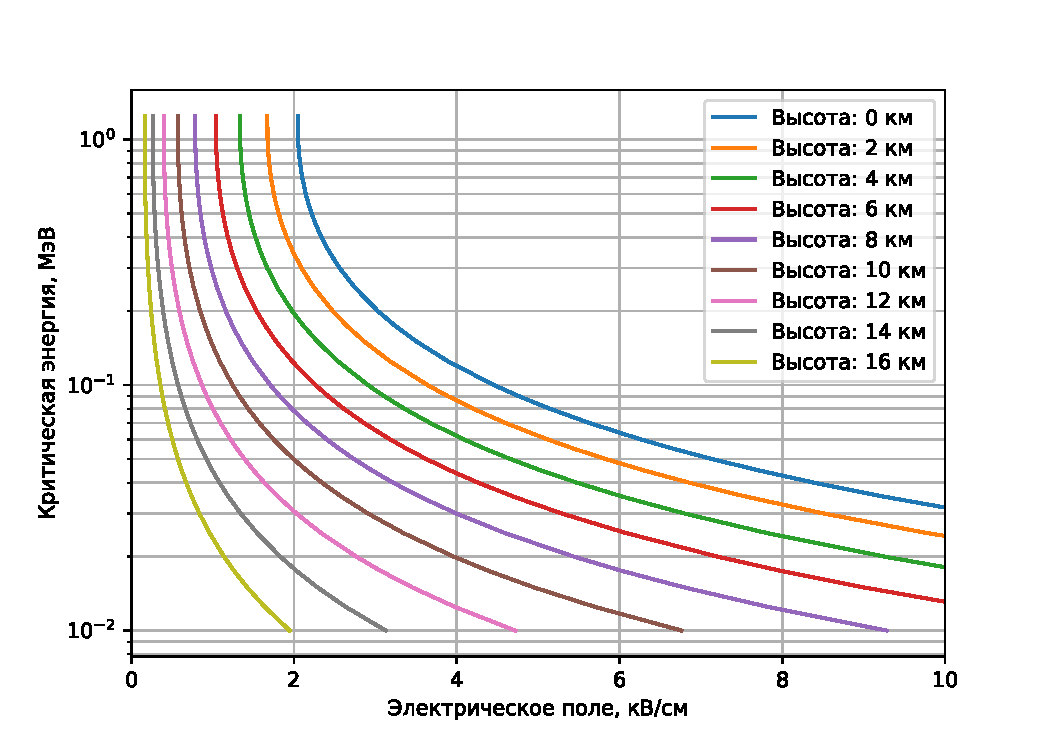
\includegraphics[width=\linewidth]{thunderstorm/02_CriticalEnergy.pdf}   \\ б)}
        \end{minipage}
        \caption{а) Сравнение критической энергии рассчитанной на основе ионизационных потерь и Монте-Карло моделирования. б) placeholder}
    \end{center}
    \label{fig:storm:simcrit}
\end{figure}

\section{Расчет числа убегающих электронов}\label{sec:thunderstorm/rrea}





Несмотря на то что есть достаточно консистентные оценки количества частиц в лавинах убегающих электронов~\cite{moss2006, DwyerSmith2005, skeltved2014, Gurevich2001ufn, Dwyer2012}, отдельные авторы~\cite{Oreshkin_2018} дают на порядки превосходящие оценки. Что бы уточнить этот вопрос, мы проведем собственные расчеты. Простая аналитическая оценка числа убегающих электронов может быть получена из элементарной теории ПУЭ~\cite{Gurevich2001ufn}. Давайте рассмотрим развитие электронной лавины в однородном электрическом поле. Согласно~\cite{Gurevich2001ufn} число убегающих электронов в RREA возрастает экспоненциально вдоль оси z:
\begin{equation}
\label{storm:exp}
N(z) = N_0 \cdot e^{\frac{z}{l_a}},
\end{equation}
где $l_a$ --- характерная длина нарастания электронной лавины, которая может быть оценена по следующей формуле:
\begin{equation}
l_a = a\frac{2 m c^{2}}{e} \frac{1}{E},
\end{equation}
где $m$ --- масса электрона, $c$ --- скорость света, константа $a \approx 11$, $E$ --- электрическое поле (для электронов с энергиями выше 80 МэВ, начинают доминировать радиационные потери, но тем не менее эта формула может дать оценку сверху). В качестве альтернативы мы можем использовать эмпирическую формулу полученную в стимуляциях Дуайера~\cite{Dwyer2007}:
\begin{equation}
\label{storm:dwyer}
l_a = \frac{7300 kV}{E - 276 \frac{kV}{m} \cdot \frac{n}{n_0}},
\end{equation}
где $E$ --- электрическое поле, $n$ - концентрация воздуха, $n_0$ --- концентрация воздуха при н. у. Используя эти формулы, можно рассчитать число релятивистских электронов в зависимости от размера области с поле и величины поля. Результаты расчетов для высоты 10~км представлены на графике ~\ref{storm:number_runway}а, из него видно для максимально возможных условий на данной высоте (регион с полем не превышает 1200~метров, а электрическое поле~200 кВ/м) количество электронов не превышает $10^{10}$.

\begin{figure}[t]
    \begin{center}
        \begin{minipage}[h]{0.49\linewidth}
            \center{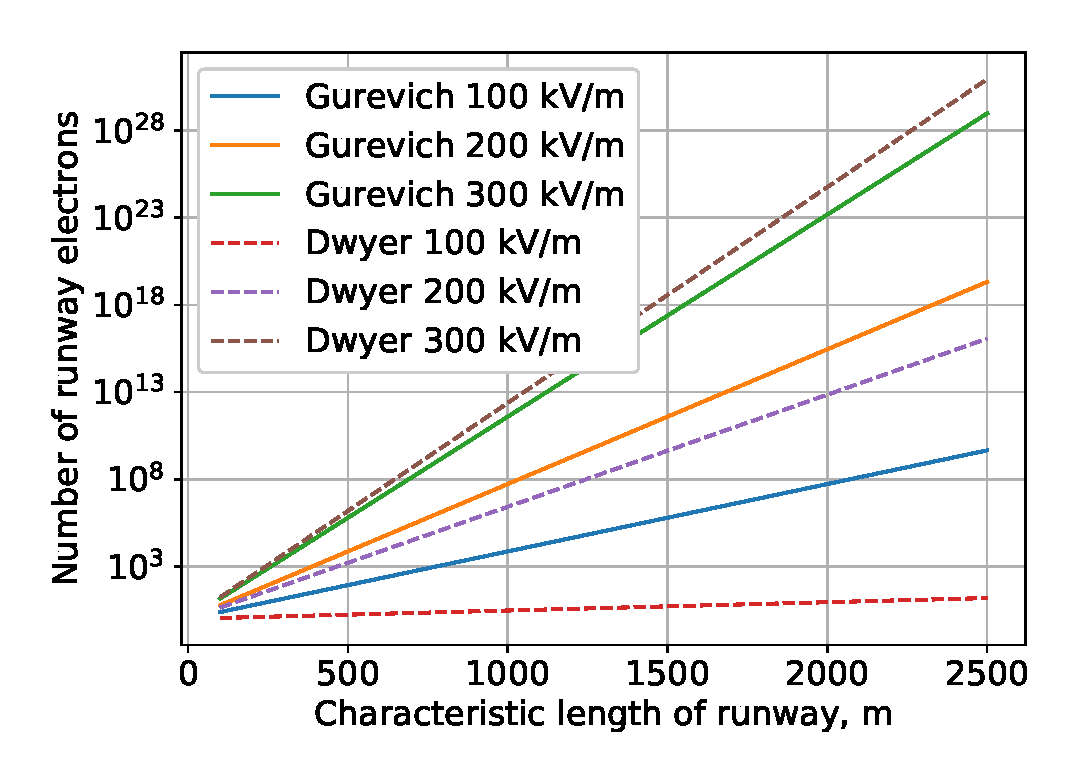
\includegraphics[width=\linewidth]{thunderstorm/epl2020/gurevich.eps} \\ а)}
        \end{minipage}
        \hfill
        \begin{minipage}[h]{0.49\linewidth}
            \center{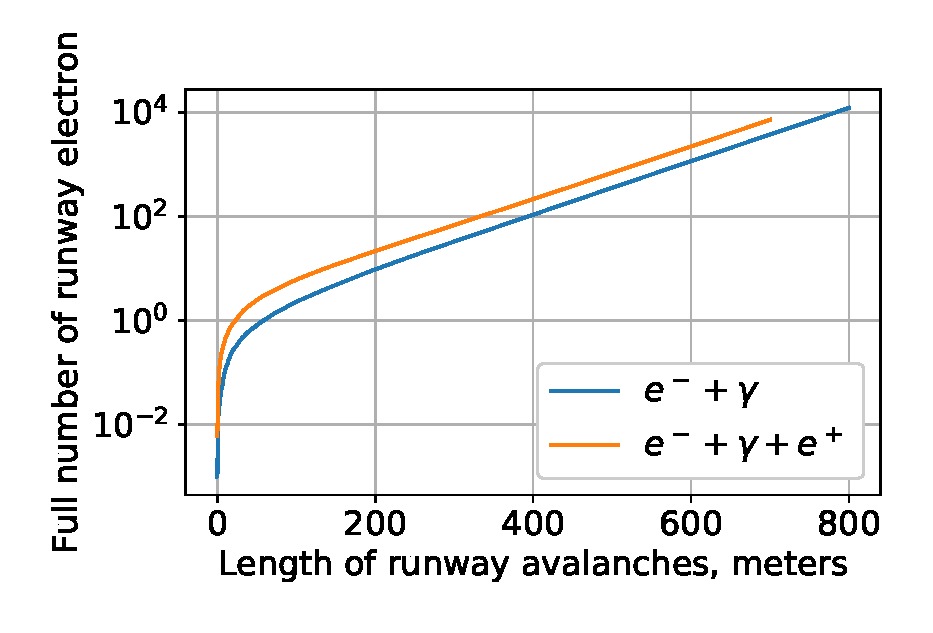
\includegraphics[width=\linewidth]{thunderstorm/epl2020/simulation.eps}   \\ б)}
        \end{minipage}
        \caption{  а) Число убегающих электронов в лавине в зависимости от длинны лавины. б) Число убегающих электронов из GEANT4 симуляции: синяя линия --- симуляция без позитронов, оранжевая --- с позитронами.}
    \end{center}
    \label{storm:number_runway}
\end{figure}
Более точные значения можно получить с помощью Монте-Карло моделирования лавины в электрическом поле с помощью GEANT4~\cite{Geant2003,Geant2006, Geant2016} (в данном разделе приведены расчеты с использованием версии 4.10.05).
Моделирование было проведено для следующих параметров: 
\begin{itemize}
    \item Область с полем представляет собой  цилиндр с шириной много большей его толщины, электрическое поле и плотность воздуха однородны;
    \item Плотность воздуха --- 0.4~кг/м~$^3$ (соответствует атмосферному давлению в  $\sim 0.25$~атм или высоте 10~км от уровня моря);
    \item Электрическое поле --- $200$~кВ/м (это максимальное электрическое поле обычно измеряемое в облаках~\cite{rakov_uman});
    \item Размер области с полем --- $800$~м для симуляции без позитронов и $700$~м для симуляции с позитронами (как мы увидим позже эти длины примерно соответствуют 10 характерным длинам нарастания лавины, что позволяет признать эти длины достаточными);
    \item Минимальный порог для рождения частиц --- 0.05 МэВ.
\end{itemize}
В каждой симуляции запускалось 1000 затравочных электронов (конечные результаты приведены на один электрон), результат симуляции приведен на рисунке~\ref{storm:number_runway}б. Результаты были фитированы функцией ~\ref{storm:exp}, в результате чего получены значения  $l_a \approx 85 m$ для симуляции без позитронов и $l_a \approx 78~m$ для симуляции с позитронами (для сравнения ~Eq.~\ref{storm:dwyer}~(формула Дуайера) предсказывает $l_a \approx 64~m$, причины вызывающие различие с формулой Дуайера будут рассмотрены в~\ref{sec:thunderstorm/rdfm}). Используя полученную характерную длину можно оценить число убегающих электронов для разных длин, некоторые характерные значения приведены в таблице~\ref{tab:storm:approx}. На интересном нам участке $1200 - 1700$~метров рождает только $10^6-10^8$ убегающих электронов, что гораздо меньше числа $10^{16}$ предсказываемого в работе~\cite{Oreshkin_2018}, и сравнимо с оценками даваемыми другими авторами.
\begin{table}[h]
    \centering
    \begin{tabular}{crrr}
        \hline
        & & \multicolumn{2}{r}{Число убегающих электронов} \\
        &   Длина, м &   без позитронов &  с позитронами \\
        \hline
        \multirow{4}*{\rotatebox[origin=c]{90}{моделирование}} & 300 &  34.3      &  46 \\
        & 500 &  361     &  589 \\
        & 700 &  3802     &  7539 \\
        & 800 &  12350 &  --- \\
        \hline
        \multirow{5}*{\rotatebox[origin=c]{90}{экстраполяция}}& 1200 &  1.4e+06 &  4.3e+06 \\
        & 1700 &  5.0e+08 &  2.5e+09 \\
        & 2000 &  1.7e+10 &  1.2e+11 \\
        & 4000 &  2.9e+20 &  1.3e+22 \\
        & 5000 &  3.7e+25 &  4.5e+27 \\
        \hline
    \end{tabular}
    \caption{Оценка полного числа убегающих электронов основанная на симуляции в области размером 700-800 метров. Первая часть таблицы это взятые из симуляции, вторая часть это экстраполяция результатов моделирования.}
    \label{tab:storm:approx}
\end{table}

Результаты моделирования представлены в статье~\cite{zelenyi_2020}.

\clearpage